\section{Results}

Our analysis of the National Vulnerability Database (NVD) yielded a comprehensive dataset that allows us to profile security faults across multiple dimensions. Following the methodology outlined in Phase II, we present the results of our data collection and analysis, addressing the research question of how software security faults profile regarding software type, technology, causes, and programming language.

\subsection{How do vulnerability patterns differ across software types?}

To understand how vulnerability patterns vary by software type, we analyzed the 100\%‐stacked distribution of the top CWEs across seven categories of software products (extension, framework, library, mobile\_app, server, utility, web\_application). This analysis builds on the consolidated dataset of 55,657 CVEs for which software type was determined, after mapping products to types and programming languages as described in the methodology.

Figure~\ref{fig:sw_typ_cwe} (100\%‐stacked bar chart) shows the relative frequency of four prominent CWEs (CWE-352: Cross-Site Request Forgery; CWE-787: Out-of-Bounds Write; CWE-79: Cross-Site Scripting; CWE-89: SQL Injection) along with “Others” (all remaining CWEs) for each software type. The key observations are as follows:

\begin{figure}[!h]
	\centering
    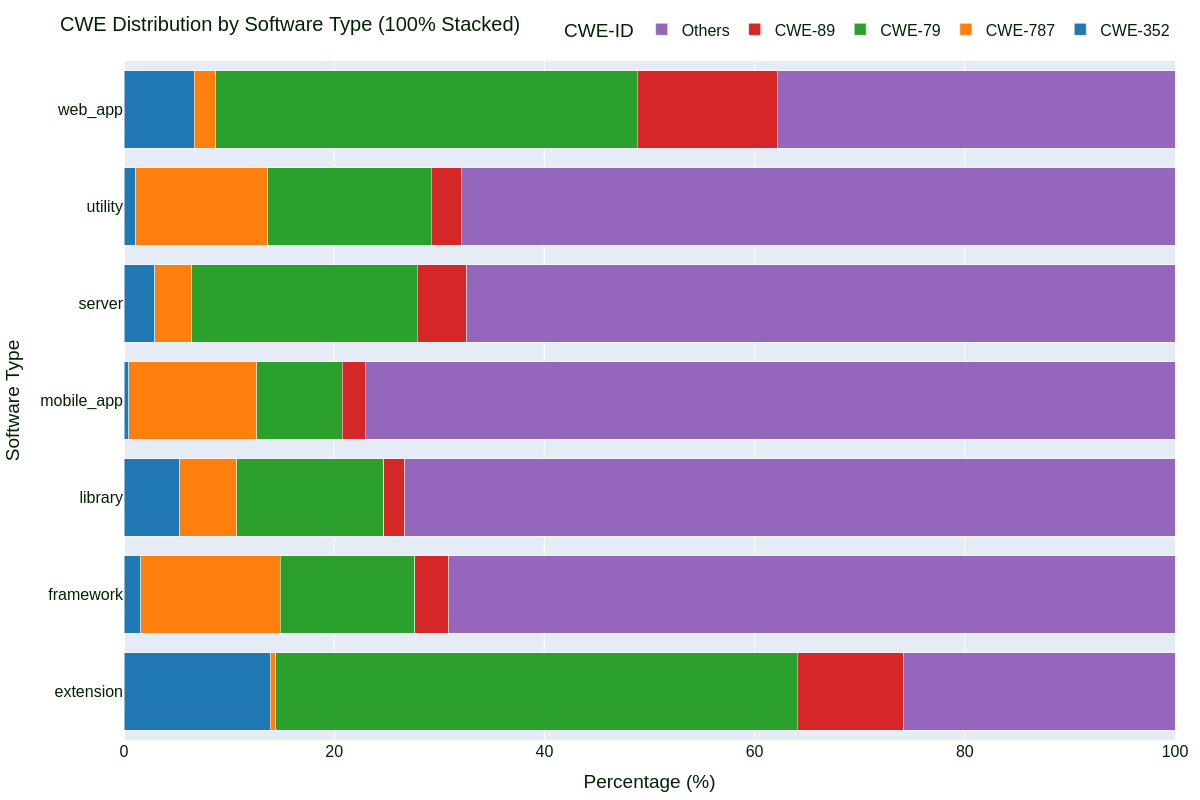
\includegraphics[width=0.95\textwidth]{figures/chapter_2/stacked_bar_software_cwe.png}
	\caption{100\%‐stacked bar chart of CWE Distribution by Software Type}
	\label{fig:sw_typ_cwe}
\end{figure}

\begin{itemize}
    \item \textbf{Extensions}: Nearly half of the vulnerabilities in extensions are XSS (CWE-79: 49.6\%), followed by CSRF (CWE-352: 13.9\%) and SQL Injection (CWE-89: 10.2\%), with a substantial residual portion (25.8\%) in “Others.” This suggests that browser or plugin-like components are predominantly exposed to web-based injection and script injection flaws, likely due to their frequent interaction with untrusted web content or APIs.
    \item \textbf{Web Applications}: Web applications similarly exhibit a high proportion of XSS (40.1\%) and SQL Injection (13.3\%), with CSRF accounting for 6.7\% and “Others” comprising 37.9\%. This aligns with expectations for web-facing services, where input validation and session/state management issues are primary concerns.
    \item \textbf{Servers}: Server software shows a moderate share of XSS (21.5\%) and lower SQL Injection (4.7\%) and CSRF (2.9\%), with “Others” at 67.4\%. The lower injection percentages may reflect that many server-side components rely on different interfaces (e.g., APIs, network protocols) where other types of weaknesses (captured in “Others”) predominate.
    \item \textbf{Frameworks}: Frameworks stand out with a notable portion of memory-related issues (CWE-787: 13.3\%), alongside XSS (12.8\%) and a large “Others” category (69.1\%). This indicates that underlying libraries or platforms (e.g., web frameworks, application frameworks) face both input-handling flaws and lower-level implementation bugs, including memory safety vulnerabilities.
    \item \textbf{Libraries}: Libraries have a smaller fraction of XSS (14.0\%) and Out-of-Bounds Write (5.4\%), with most vulnerabilities falling into “Others” (73.3\%). This diffuse distribution suggests libraries span a wide range of functionality, so specific weakness patterns vary greatly depending on the domain (e.g., cryptography, data processing, image handling).
    \item \textbf{Utilities}: Utility software shows a moderate XSS share (15.6\%) and a higher proportion of Out-of-Bounds Write (12.5\%), with “Others” at 67.9\%. Utilities (e.g., command-line tools, system utilities) often involve file or memory operations, which may explain the relative prominence of memory-related flaws alongside occasional script or injection issues when utilities process complex inputs.
    \item \textbf{Mobile Applications}: Mobile apps exhibit a small fraction of XSS (8.1\%) but a notable Out-of-Bounds Write share (12.2\%), with “Others” dominating (77.0\%). This pattern reflects that while mobile apps may embed webviews (leading to some XSS), many vulnerabilities arise from platform-specific memory handling or misuse of APIs.
\end{itemize}

Overall, software types with strong web-facing components (extensions, web applications) show high proportions of injection and scripting weaknesses, whereas types closer to system-level or framework-level code (frameworks, utilities, mobile apps) surface more memory-related issues. Libraries cover a broad spectrum, resulting in a large “Others” bucket. Servers lie in between, with diverse vulnerabilities but fewer classical web injection flaws.

\begin{boxC}
\textit{\textbf{Finding 1.} Vulnerability patterns vary significantly by software type: web-facing contexts (extensions, web applications) are dominated by script- and injection-related weaknesses (e.g., XSS, SQL Injection), while frameworks, utilities, and mobile applications exhibit higher rates of memory safety issues (e.g., out-of-bounds writes). Libraries show diffuse patterns across many weakness types. This implies that security mitigations should be tailored to software type, emphasizing input validation and sanitization for web components, and memory safety practices for frameworks and system-oriented software.}
\end{boxC}

\subsection{How do programming languages correlate with security faults?}

Our language mapping process successfully identified the primary programming language for 13,081 vulnerable software products. The distribution reveals several key insights:

\begin{itemize}
    \item Web-oriented languages dominate the vulnerability landscape, with PHP (32.4\%, 4,236 samples) and JavaScript (13.9\%, 1,824 samples) accounting for nearly half of all identified vulnerabilities.
    \item Java (10.8\%, 1,415 samples) represents a significant portion, reflecting its widespread use in enterprise applications.
    \item Systems programming languages like C (6.8\%, 887 samples) and C++ (3.4\%, 448 samples) show fewer vulnerabilities in absolute numbers but may represent more severe issues when they occur.
    \item Modern languages like Python (6.2\%, 817 samples), Go (3.8\%, 496 samples), and Rust (2.0\%, 267 samples) are present but with lower frequency, potentially indicating better security properties or less widespread adoption.
\end{itemize}

The predominance of PHP and JavaScript vulnerabilities aligns with their extensive use in web development, where exposure to user input creates numerous attack vectors. The relatively lower representation of systems languages may reflect either better security practices or the challenges in vulnerability discovery for these languages.

\subsection{Common Weakness Enumeration (CWE) Analysis}

Our analysis extracted 18,566 CVE entries with associated CWE identifiers, revealing the most common vulnerability types:

\begin{itemize}
    \item Cross-Site Scripting (CWE-79) dominates with 32.3\% (6,000 samples) of all vulnerabilities, highlighting the persistent challenge of securing user input in web applications.
    \item Cross-Site Request Forgery (CWE-352, 7.7\%, 1,434 samples) and SQL Injection (CWE-89, 7.1\%, 1,316 samples) represent the next tier of common web vulnerabilities.
    \item Path Traversal (CWE-22, 4.8\%, 899 samples) and Authorization Issues (CWE-862, 3.9\%, 727 samples) round out the top five.
    \item Memory corruption vulnerabilities like Out-of-bounds Write (CWE-787, 3.6\%, 661 samples) and Out-of-bounds Read (CWE-125, 2.3\%, 422 samples) appear less frequently but often represent higher severity issues.
\end{itemize}

The prevalence of web-related vulnerabilities (CWE-79, CWE-352, CWE-89) reflects the extensive attack surface of web applications and the challenges in properly validating and sanitizing user input. Memory corruption vulnerabilities, while less common, remain a persistent threat, particularly in systems programming contexts.

\subsection{Multi-dimensional Vulnerability Profiling}

The consolidated dataset (18,566 samples total, including 7,868 products with both language and software type identified) reveals important patterns across software types, programming languages, and vulnerability classes:

\begin{itemize}
    \item PHP-based extensions and web applications are particularly susceptible to Cross-Site Scripting (CWE-79), with 2,175 and 1,450 instances respectively, representing the most common vulnerability profiles.
    \item Cross-Site Request Forgery (CWE-352) is also prevalent in PHP extensions (607 instances) and web applications (334 instances).
    \item SQL Injection (CWE-89) affects PHP web applications (477 instances) and extensions (399 instances) most frequently.
    \item JavaScript applications show significant vulnerability to Cross-Site Scripting (CWE-79, 245 instances), while Java libraries exhibit both XSS (221 instances) and CSRF (188 instances) vulnerabilities.
    \item Memory corruption vulnerabilities cluster in C-based frameworks (CWE-787, 158 instances; CWE-125, 147 instances) and utilities (CWE-125, 154 instances; CWE-787, 138 instances).
\end{itemize}

These patterns reveal distinct vulnerability profiles across the software ecosystem:

\begin{enumerate}
    \item \textbf{Web Application Profile:} Dominated by input validation vulnerabilities (XSS, CSRF, SQLi) in PHP and JavaScript applications, particularly in extensions and web applications.
    \item \textbf{Systems Software Profile:} Characterized by memory corruption issues (buffer overflows, use-after-free) in C and C++ utilities and frameworks.
    \item \textbf{Enterprise Application Profile:} Represented by a mix of web vulnerabilities and authorization issues in Java libraries and frameworks.
\end{enumerate}

\subsection{Addressing the Research Question}

Returning to our research question—\textit{How do software security faults profile regarding software type, technology, causes, and programming language?}—our analysis reveals several key insights:

\begin{itemize}
    \item \textbf{Software Type:} Extensions and web applications are most vulnerable to input validation issues, while utilities and frameworks show greater susceptibility to memory corruption. Servers exhibit a more diverse vulnerability profile spanning both categories.

    \item \textbf{Technology:} Web technologies dominate the vulnerability landscape, with client-side (XSS, CSRF) and server-side (SQLi, path traversal) issues being most prevalent.

    \item \textbf{Causes:} Improper input validation emerges as the dominant root cause across the ecosystem, followed by memory management issues in systems software and authorization problems across multiple software types.

    \item \textbf{Programming Language:} Strong correlations exist between languages and vulnerability types: PHP and JavaScript with web vulnerabilities, C and C++ with memory corruption, and Java with a mix of web and authorization issues.
\end{itemize}

These findings demonstrate that vulnerability profiles are not uniform across the software ecosystem but rather cluster into distinct patterns based on software type, implementation language, and application domain. This multi-dimensional profiling provides a more nuanced understanding of security fault distribution than previous single-dimensional analyses.
